\documentclass{beamer}

\usepackage[american,russian]{babel}

\usefonttheme{serif}

\setbeamertemplate{footline}[frame number]{}
\setbeamertemplate{navigation symbols}{}

\usecolortheme{default}
\setbeamercolor{block title}{bg=lily!20,fg=black}
\setbeamercolor{block body}{bg = blue!10, fg = black}
\setbeamertemplate{itemize item}[square]
\setbeamercolor{itemize item}{fg = cyan}
\setbeamercolor{enumerate item}{fg = cyan}

\usetheme{default}
\usepackage[justification=centering]{caption}

%\setbeamercolor{titlelike}{fg=cyan}
%Information to be included in the title page:

\title[About Beamer] %optional
{Optical Breakdown}

%\subtitle{A short story}

\author[Arthur, Doe] % (optional, for multiple authors)
{A. Simankovich \and D. Dedkov }

\institute[VFU] % (optional)
{
	Moscow Institute of Physics and Technology
}

\date[VLC 2023] % (optional)
%{Very Large Conference, April 2021}

%\logo{\includegraphics[height=1cm]{overleaf-logo}}

\begin{document}
	
	\frame{\titlepage}
	
	\begin{frame}
		\frametitle{Abstract}
		
		Article studies optical breakdown effect in focused laser radiation. Theoretical description of breakdown formation in gases provided. Spectra and oscillograms of breakdown spark measured in different substances. Threshold fields are estimated.
	\end{frame}
	
	
	\begin{frame}[plain,c]
		
		\begin{center}
			\huge \usebeamercolor[fg]{frametitle} Introduction
		\end{center}
		
	\end{frame}
	
	
	\begin{frame}
		\frametitle{Static electrical breakdown}
		
		\begin{figure}
			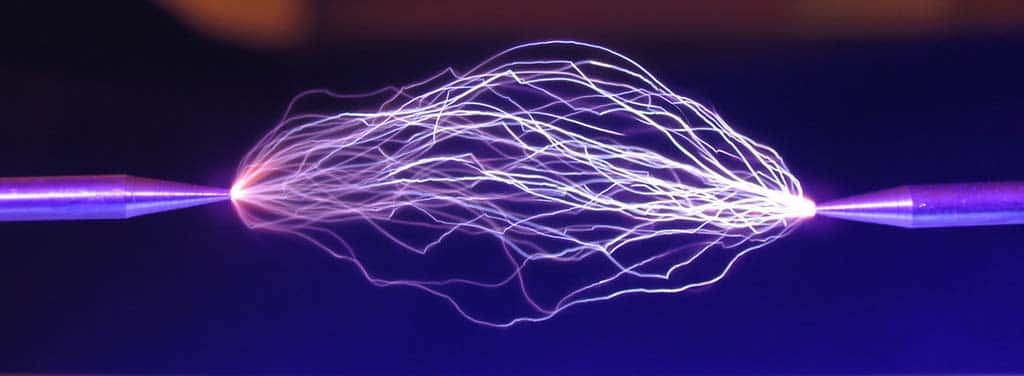
\includegraphics[width=0.8\linewidth]{res/const_discharge.jpg}
		\end{figure}
		
		\begin{columns}
			\column{0.6\linewidth}
			\begin{figure}
				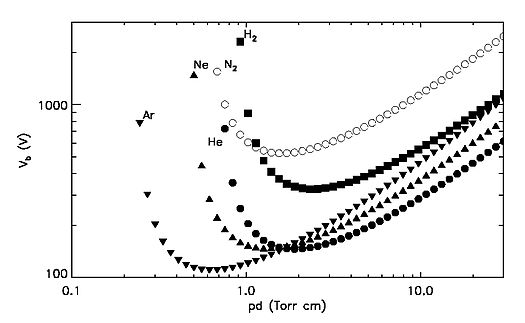
\includegraphics[width=\linewidth]{res/paschen.jpg}
			\end{figure}
			
			\column{0.5\linewidth}
			Paschen's law describes static electrical breakdown.
		\end{columns}
		
		%			Самый известный и хорошо изученный тип пробоя -- пробой постоянным напряжением. Его поведение в первом приближении описывается кривыми Пашена.
		%			Заметим, что у кривой существует минимум.	
	\end{frame}
	
	\begin{frame}
		\frametitle{Alternating-field electrical breakdown}
		
		\begin{columns}
			\column{0.15\linewidth}
			\begin{figure}
				\centering
				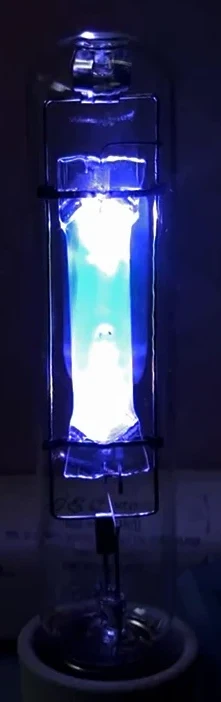
\includegraphics[width=1\linewidth]{res/hg_lamp.png}
				\caption*{Mercury lamp}
			\end{figure}
			
			\column{0.7\linewidth}
			\begin{figure}
				\centering
				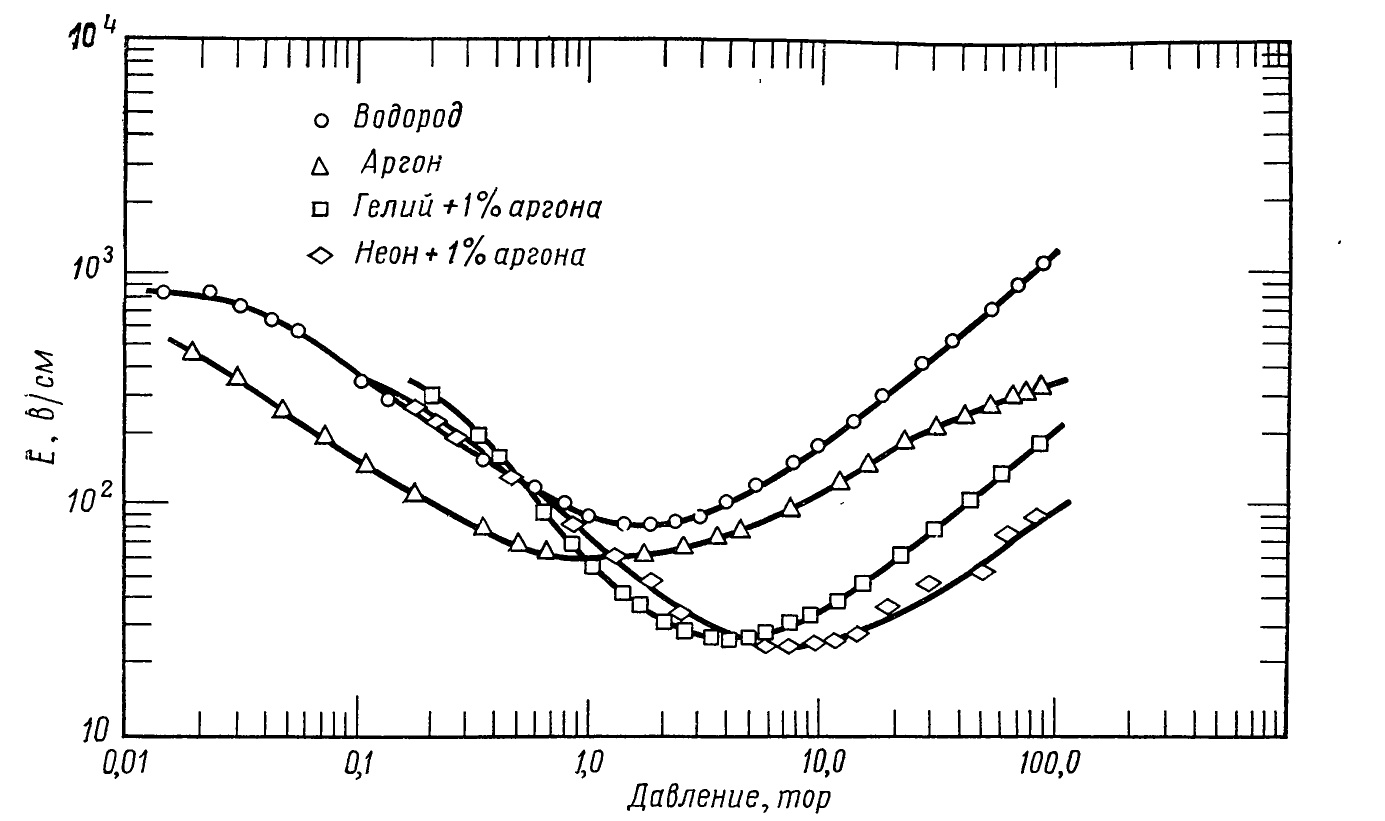
\includegraphics[width=1\linewidth]{res/microwave_discharge.png}
				\caption*{Threshold field on pressure\\ ($f = 992$ MHz, diffusion length $0.631$ cm)}
			\end{figure}
			
		\end{columns}		
		
		%TODO: ссылка на Microwave Breakdown in Gases by A. D. MacDONALD
		Alternating field also induces breakdown.
		
		%		Под действием переменного поля также возникает пробой. Его минимум для типичных параметров установки расположен в диапазоне давлений, близких к нормальному.
	\end{frame}
	
	\begin{frame}
		\frametitle{Optical breakdown}
		\begin{columns}
			\column{0.4\linewidth}
			\begin{figure}
				\centering
				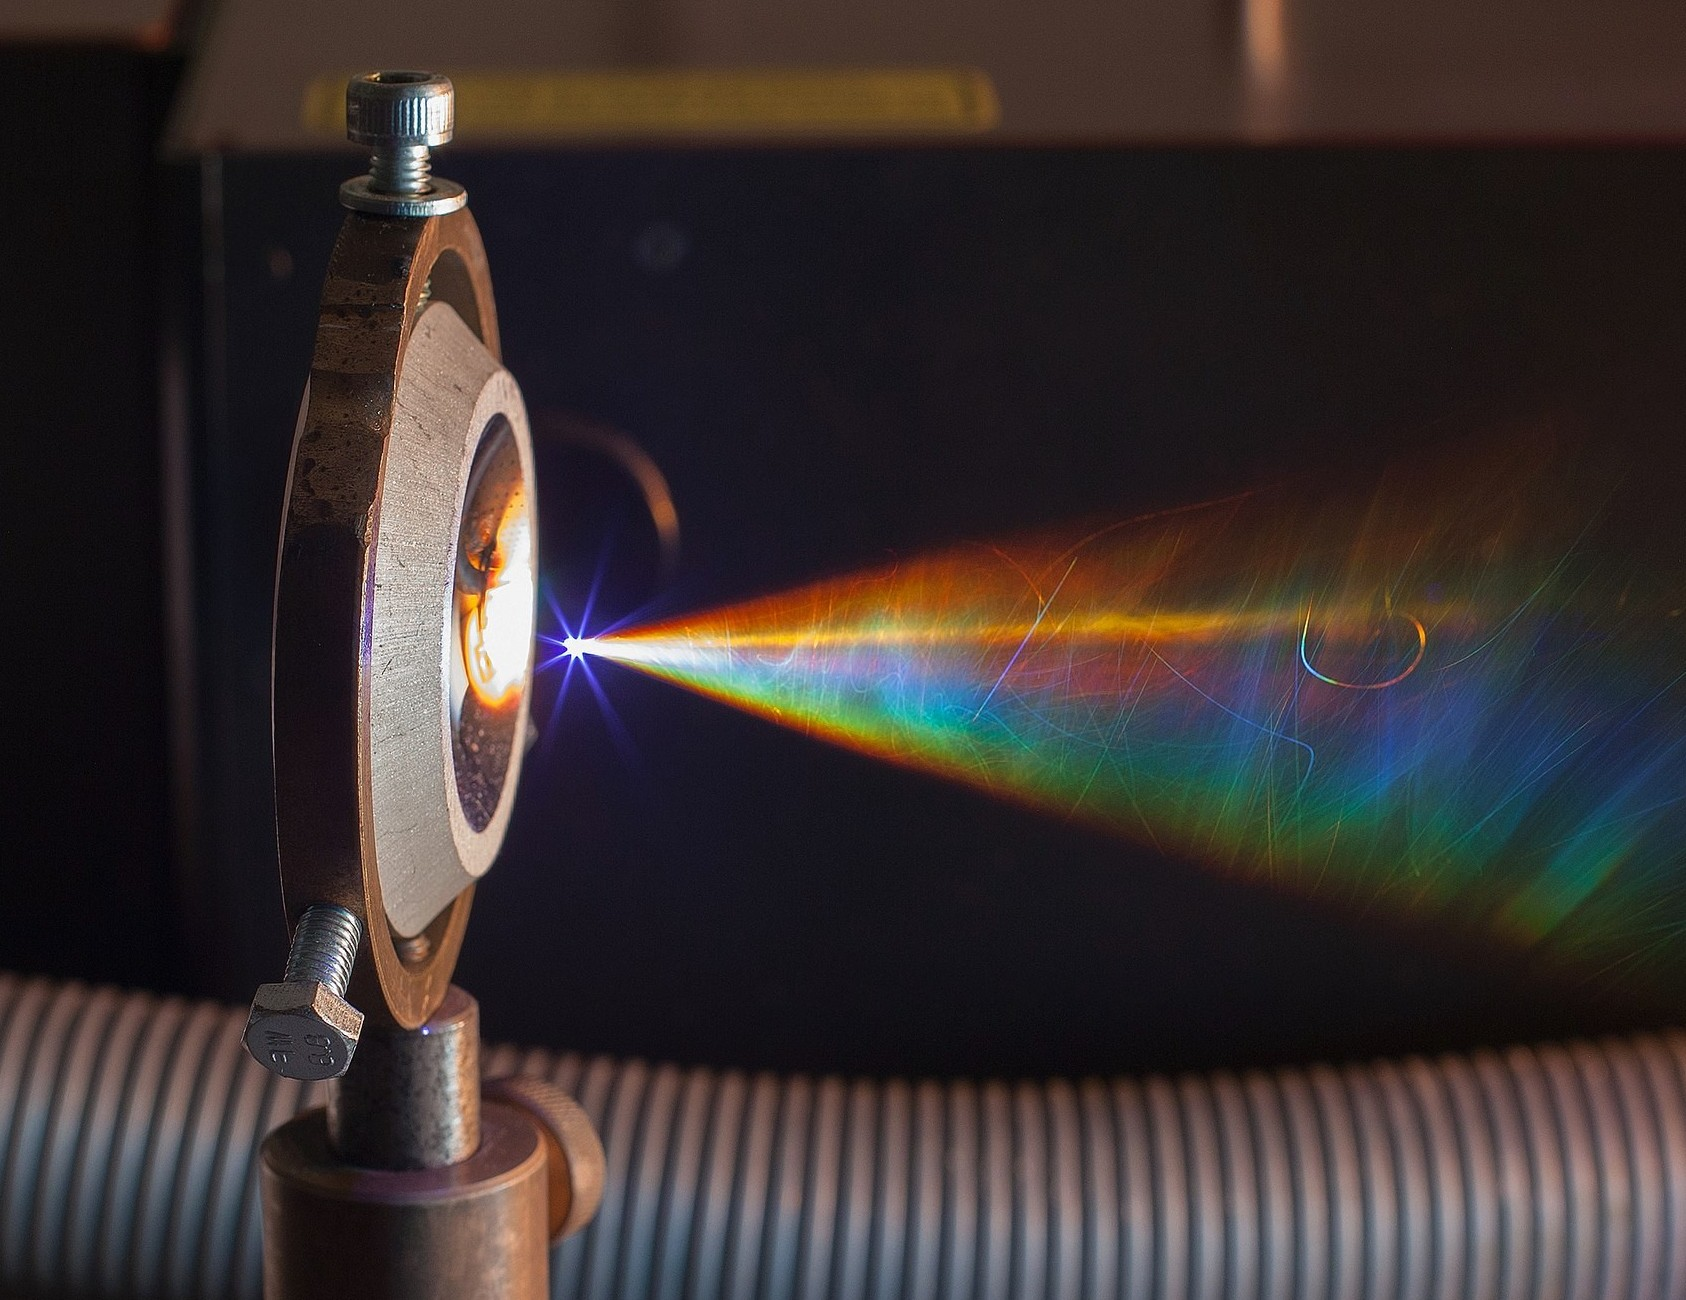
\includegraphics[width=1.05\linewidth]{res/new_femtosecond_laser_spark.jpg}
				\caption*{Femtosecond laser air breakdown}
			\end{figure}
			
			\column{0.6\linewidth}
			\begin{figure}
				\centering
				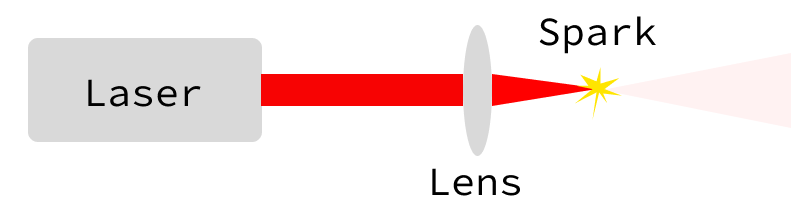
\includegraphics[width=1.0\linewidth]{res/scheme.png}
				\caption*{Basic scheme}
			\end{figure}
			
			
		\end{columns}
		%TODO: может не стоит вставлять картинку с непонятной радугой?
		\begin{itemize}
			\item Optical breakdown -- $E \approx 10^6 \div 10^7$ V/cm. 
			\item Static and alternating field -- $E \approx 3 \cdot 10^4$ V/cm.
		\end{itemize}
		Charachteristic parameters:
		$$ P \approx 30 \text{ MW}, \quad d = 2 \cdot 10^{-2} \text{ cm} $$
		$$ I \approx 10^5 \text{ MW/cm}^2, \quad E \approx 6 \cdot 10^6 \text{ V/cm} $$
		
		%		В данной работе изучается пробой полем оптического диапазона. Характерные значения поля для пробоя газа $E \approx 10^6 \div 10^7$ В/см (для постоянного и СВЧ полей $E \approx 3 \cdot 10^4$ В/см). 
		
		%Такие величины полей достижимы только в фокусированном лазерном излучении: при пиковой мощности и диаметре фокуса $2 \cdot 10^{-2}$ см получаем $I \approx 10^5$ МВт/см$^2$ и поле $E = 6 \cdot 10^6$ В/см.
		
	\end{frame}
	
	\begin{frame}
		\frametitle{Optical breakdown applications}
		
		\begin{figure}
			\centering
			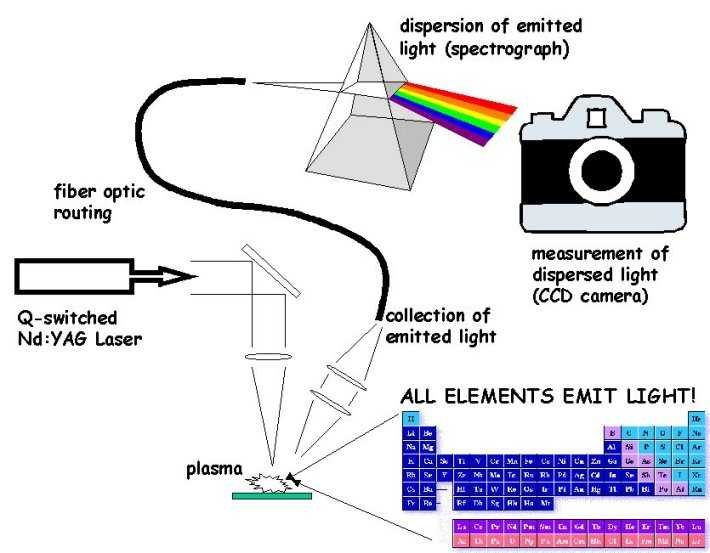
\includegraphics[width=0.5\linewidth]{res/libs.jpg}
			\caption*{Laser-Induced Breakdown Spectroscopy (LIBS)}
		\end{figure}
		
		\begin{itemize}
			\item Laser-Induced Breakdown Spectroscopy.
			\item Connected with nuclear fusion.
			\item Development of quantum theory.
		\end{itemize}
		
		%		Лазерно-искровая эмиссионная спектрометрия --  основное прикладное применение лазерного пробоя.
		%		
		%		Явление лазерного пробоя тесно связано с задачами термоядерного синтеза.
		%		
		%		Изучение лазерного пробоя позволяет получить важные выводы для квантовой теории.
	\end{frame}
	
	\begin{frame}
		\frametitle{Spark stages}
		\begin{figure}
			\centering
			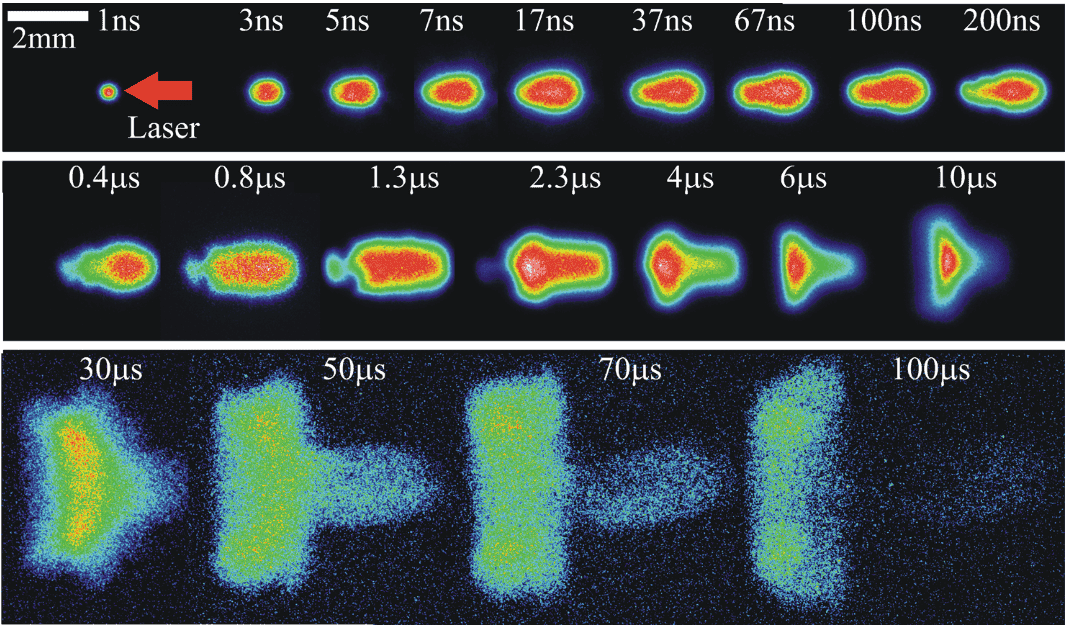
\includegraphics[width=0.8\linewidth]{res/spark_evolution.png}
			\caption*{Spark evolution in time}
		\end{figure}
		\vspace{-5pt}
		Three stages of laser spark:
		\begin{itemize}
			\item Breakdown: ionization and initial plasma formation.
			\item Plasma-photon interaction, plasma front movement.
			\item Shock wave spreading, glowing.
		\end{itemize}
	\end{frame}
	
	
	\begin{frame}[plain,c]
		
		\begin{center}
			\huge \usebeamercolor[fg]{frametitle} Theory
		\end{center}
		
	\end{frame}
	
	\begin{frame}
		\frametitle{Breakdown initiation -- ionization by radiation}
		\vspace{-5pt}
		Two mechanisms of electron ejection by radiation:
		% TODO: А может в постоянном поле быть "просто достаточное поле", чтобы быть сильнее притяжения электрона к ядру? Это тоже туннельный эффект?
		\begin{columns}
			\column{0.5\linewidth}
			\begin{figure}
				\centering
				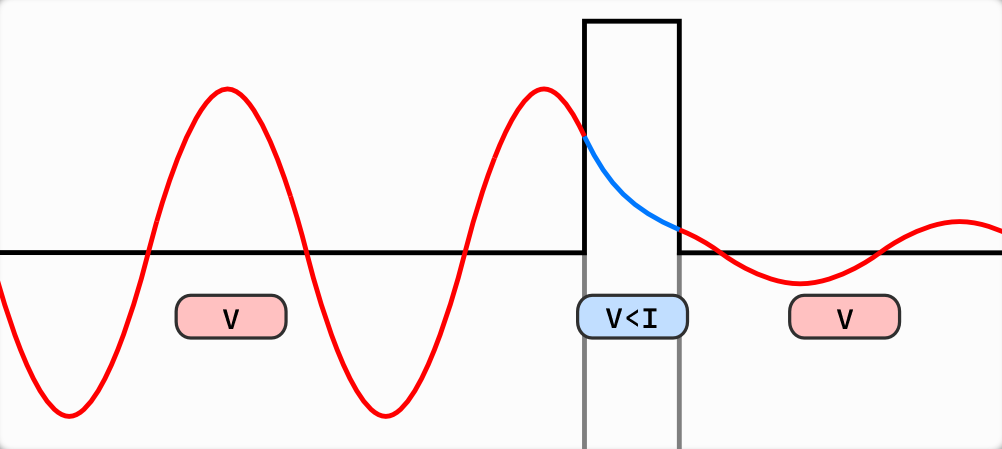
\includegraphics[width=\linewidth]{res/tunneling.png}
				\caption*{Quantum tunneling}
			\end{figure}
			\vspace{-10pt}
			\footnotesize
			\begin{itemize}
				\setlength\itemsep{-2pt}
				\item $E$ -- lightwave field.
				\item $I$ -- ionization energy.
				\item $\Delta \sim \frac{I}{eE}$ -- potential barrier width.
				\item $v \sim \sqrt{I/m}$ -- electron velocity.
				\item $\tau \sim \Delta / v \sim \frac{\sqrt{Im}}{eE}$ -- electron time-of-flight of barrier.
			\end{itemize}
			$$\omega \tau \ll 1 \text{ -- 'static' field condition.}$$
			
			\column{0.5\linewidth}
			\begin{figure}
				\centering
				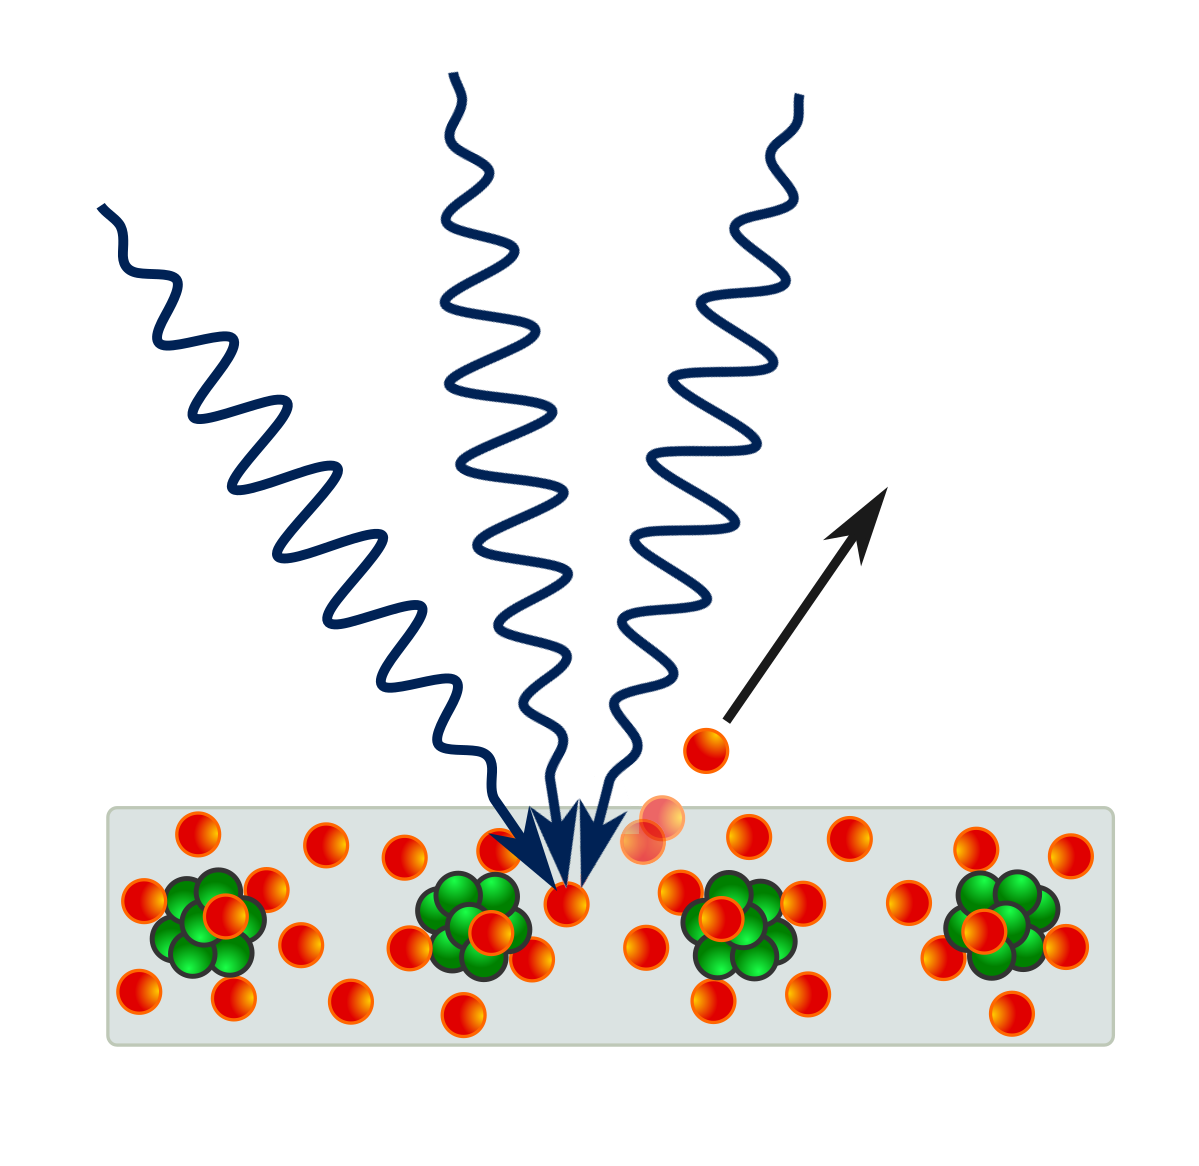
\includegraphics[width=0.7\linewidth]{res/multiphoton.png}
				\caption*{Multiquantum photoelectric effect}
			\end{figure}
			\footnotesize
			$\omega \tau \gg 1$ -- condition of many quanta absorption on oscillation.
		\end{columns}
		\vspace{10pt}
		Estimation on optical frequencies gives $\omega \tau \gg 1$.
		%Для вырывания электрона из атома есть два механизма: туннельный эффект (например, в статическом электрическом поле) и многоквантовый фотоэффект.
		%Ширина потенциального барьера под действием поля $E$ составляет $\Delta \sim \frac{I}{eE}$. Скорость электрона $v \sim \sqrt{I/m}$. Тогда время пролета барьера $\tau \sim \Delta / v \sim \frac{\sqrt{Im}}{eE}$. Туннелирование может происходить если поле остается 'стационарным' во время пролета барьера: $\omega \tau \ll 1$. Для многоквантовости требуется обратное неравенство: $\omega \tau \gg 1$. Для типичных значений лазерного излучения характерно $\omega \tau \gg 1$.
		
	\end{frame}
	
	\begin{frame}
		\frametitle{Multiquantum photoeffect probability}
		\begin{itemize}
			\setlength\itemsep{-2pt}
			\item $w$ -- multiquantum photoeffect probability
			\item $n$ -- number of absorbed photons
			\item $S$ -- light intensity
		\end{itemize}
		
		$w \sim S \sim E^2$ -- proportional to intensity.

		$w \sim \frac{1}{I}$ -- higher ionization energy implies lower probability.
		
		$w \sim \frac{1}{\omega}$ -- lower frequency implies more time to absorb photons.
		
		$w \sim (...)^n$ -- $n$-fold absorption.
		
		$$ w \sim \left(\frac{E^2}{\omega I}\right)^n$$
		
		According to quantum mechanics L.V.Keldysh obtained:
		\begin{equation}
			w = B \omega n^{3/2} \left(\frac{\overline{e} e^2 E^2}{8m \omega^2 I}\right)^n
		\end{equation}
		%Вероятность многоквантового фотоэффекта $w$ с поглощением $n$ фотонов пропорциональна $n$-ой степени потока квантов $w \sim F^n$, то есть $w \sim E^{2n}$.
		%$w \sim \frac{1}{I^n}$ -- чем выше порог ионизации, тем ниже вероятность.
		%$w \sim \frac{1}{\omega^n}$ -- чем ниже частота поля, тем больше характерное время изменения поля, за которое электрон может поглотить нужную энергию.
		%$$ w \sim \left(\frac{E^2}{\omega I}\right)^n$$
		%Точный расчет был произведен Л.В.Келдышем с использованием квантовой механики, его результат для фотоэффекта можно аппроксимировать следующей формулой:
		%$$ w = B \omega n^{3/2} \left(\frac{\overline{e} \pi e^2}{mc} \frac{\hbar E}{\omega I}\right)^n,$$
		%где $\omega$ -- частота поля, $B$ -- константа около 1, $$\overline{e}$ -- математическая константа, $e$ -- заряд электрона, $\hbar$ -- константа Планка.
		
		%TODO: Райзер, с 15, дописать численную оценку
		%Получить формулу как-то просто не получается(
	\end{frame}
	
	\begin{frame}
		\frametitle{Threshold field estimation}
		
		Within $t_1 \approx 40 \text{ ns}$ in spot of $r \approx 2 \cdot 10^{-2}$ cm $N = 10^{13}$ electrons should appear:
		$$N = \frac{4}{3} \pi r^3 N_a t_1 w$$
		\begin{center}
			\boxed{E = \sqrt{\frac{8m\omega^2 I}{\overline{e} e^2}} \left[\frac{w}{\omega n^{3/2}}\right]^{1/2n}}
		\end{center}
		
		For argon:
		$$ E = 1.12 \cdot 10^8 \text{ V/cm -- estimation}$$
		$$ E = 2.69 \cdot 10^6 \text{ V/cm -- experiment}$$
		
	\end{frame}
	
	\begin{frame}
		\frametitle{Breakdown development -- electron avalanche}
		
		\begin{columns}
			\column{0.5\linewidth}
			\begin{figure}
				\centering
				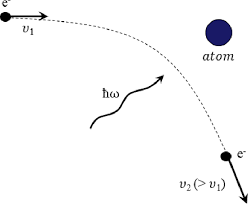
\includegraphics[width=0.7\linewidth]{res/inverse_bremsstrahlung.png}
				\caption*{Inverse bremsstrahlung}
			\end{figure}
			\column{0.5\linewidth}
			\begin{itemize}
				\item Classic: in alternating field oscillation energy converts to heat in collisions.
				\item Quantum: electron absorbs photons on collisions.
			\end{itemize}
		\end{columns}
		\begin{columns}
			\column{0.5\linewidth}
			\begin{figure}
				\centering
				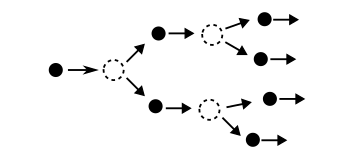
\includegraphics[width=0.8\linewidth]{res/electron_avalanche.png}
				\caption*{Electron avalanche}
			\end{figure}
			
			\column{0.5\linewidth}
			Electron avalanche develops.
			
		\end{columns}		
		
		
		% 1.
		% Под действием постоянного внешнего электрического поля свободные электроны ускоряются, при столкновении с атомом рассеивая эту энергию в тепло. В осциллирующем поле, при колебании электронов, в среднем энергия электронов при столкновениях тоже переходит в тепло (что будет показано далее).
		% Для оптического диапазона разумнее использовать квантовую теорию. При столкновениях с атомами электрон поглощает фотоны, приобретая энергию. Этот процесс обратен тормозному испусканию квантов при рассеянии.
		% Таким образом, в области поля средняя скорость электронов увеличивается. Эти электроны набирают достаточную энергию, чтобы ионизировать атомы. Новые электроны добавляются к свободным, увеличивая скорость ионизации. Формируется электронная лавина.
		
	\end{frame}
	
	\begin{frame}
		\frametitle{Breakdown development -- multiquantum photoeffect}
		
		\begin{columns}
			\column{0.5\linewidth}
			\begin{figure}
				\centering
				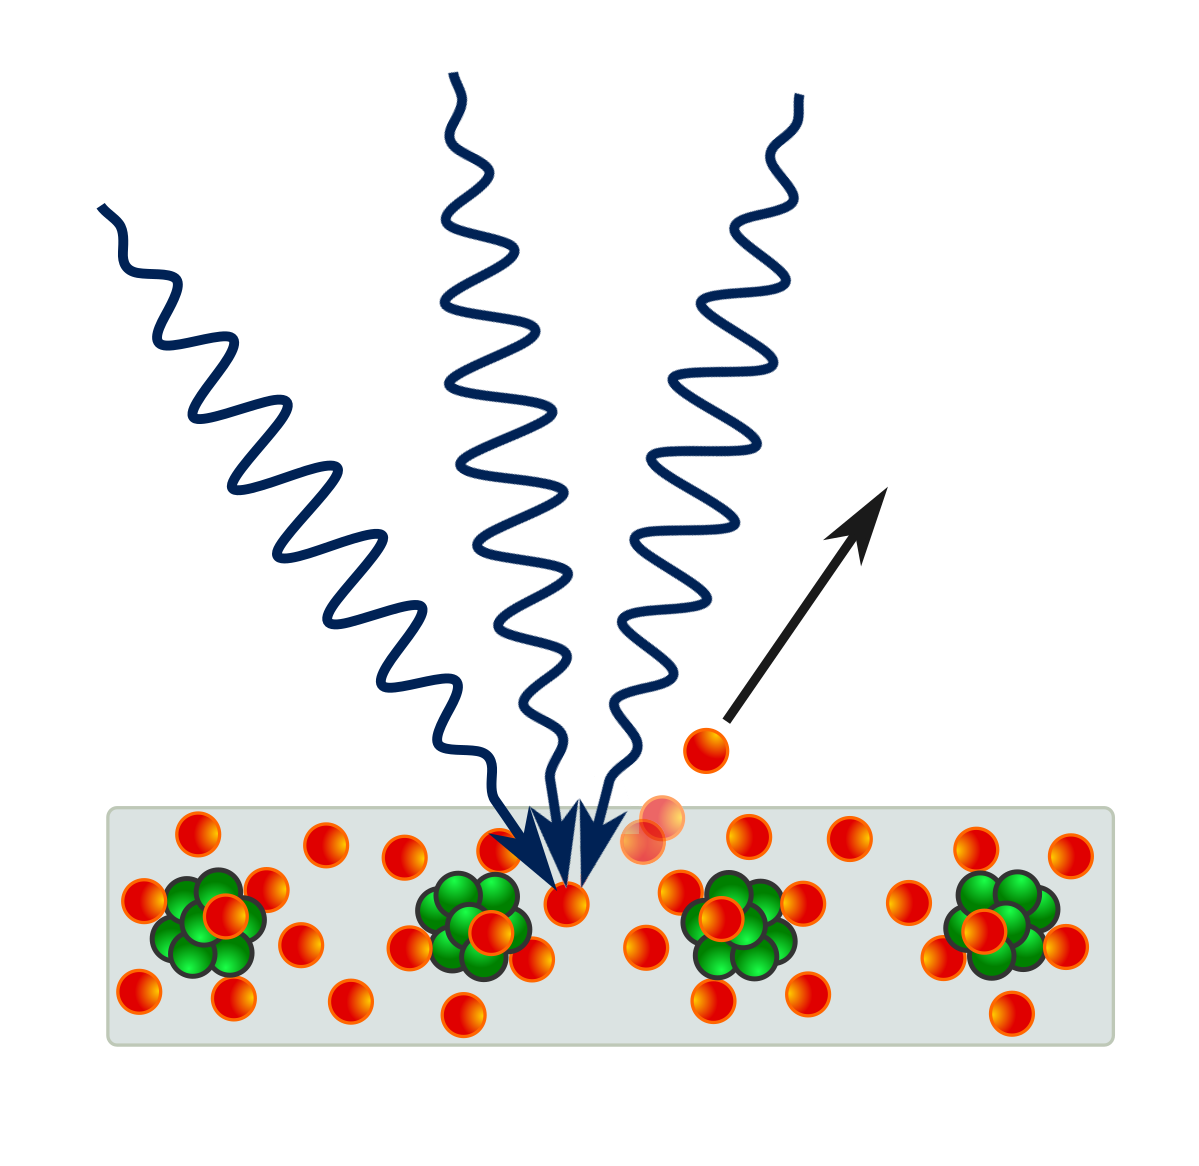
\includegraphics[width=0.9\linewidth]{res/multiphoton.png}
				\caption*{Multiquantum photoeffect}
			\end{figure}
			
			\column{0.5\linewidth}
			Electron absorbs few atoms simultaneously: 
			$$n \cdot h\nu \sim n \cdot 2 \text{ eV} > I \sim 10 \div 20 \text{ eV}$$
		\end{columns}
		
		Breakdown development:
		\begin{itemize}
			\item $p \geqslant 1\text{ atm}$ -- electron avalanche.
			\item $p \ll 1\text{ atm}$ -- multiquantum photoeffect.
		\end{itemize}
		%		Для газов при давлениях порядка атмосферного и выше -- электронная лавина.
		%		Для разреженных -- многоквантовый фотоэффект.
		% 2.
		% Вторым механизмом является многоквантовый фотоэффект. Электрон может оторваться от атома вследствие одновременного поглощения сразу нескольких фотонов. Одноквантовый эффект невозможен, так как энергия ионизации ()$I \sim 10\div20$ эВ) на порядок выше энергии фотонов видимого диапазона ($ h\nu = \sim 2$ эВ).
		% Для газов при атмосферных давлениях и выше характерен первый механизм.
	\end{frame}
	
	\begin{frame}
		\frametitle{Energy growth -- classic theory}
		%TODO: Райзер, с 19-22 (вывод довольно простой)
		
		%KEKW: Классическая теория не описывает оптический диапазон: $h\nu >> \varepsilon_{\text{кол}}$.
		
		%KEKWKEKW: А нет, описывает: $ h \nu >> \varepsilon_{\text{кол}}$, но $h\nu << \varepsilon$, а это новое условие применения классики (Райзер, с 40, 43)
		
		\begin{columns}
			\column{0.5\linewidth}
			\begin{figure}
				\centering
				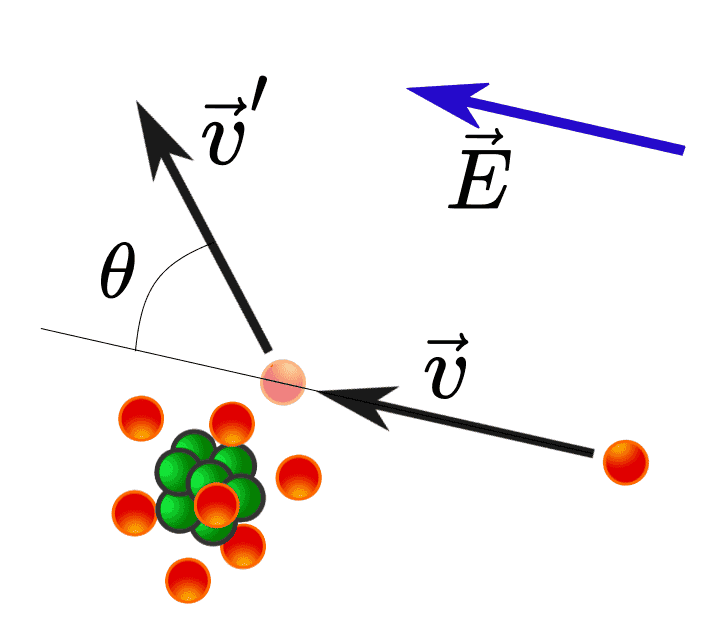
\includegraphics[width=0.8\linewidth]{res/collision.png}
				\caption*{Electron-atom collision}
			\end{figure}
			
			\column{0.5\linewidth}
			Isolated electron cannot take away field energy. Collision is essential condition.
			$$ \varepsilon_{\text{osc}} = e^2 E_0^2/4m\omega^2 \sim 0.01 \text{ eV}$$
			$$ \varepsilon \sim 10 \text{ eV} \text{ -- electron energy}$$
			\begin{center}
				\boxed{\varepsilon \gg \varepsilon_{\text{osc}} \gg h \nu}
			\end{center}
		\end{columns}
		
		Motion equation with 'friction':
		$$ m \dot{v} = - m v \nu_m - e E \qquad E = E_0 \exp(-i \omega t)$$
		$\nu_m = \nu_c (\overline{1 - \cos \theta})$ -- effective collision frequency.
		
		Work done by field on electron:
		\begin{equation}
			\boxed{d\varepsilon/dt = \frac{e^2 E^2 \nu_m}{m (\omega^2 + \nu_m^2)}
				\label{eq:energy_growth}}
		\end{equation}
		
		%		Изолированный электрон, не испытывающий столкновений с атомами, не забирает энергию у поля, получив ее лишь единожды при появлении поля. Получать энергию можно только за счет столкновений.
		%		
		%		Подразумевается, что электрон успевает набрать полную энергию колебаний $\varepsilon_{\text{кол}} = e^2 E_0^2/4m\omega^2$ за время между столкновениями.
		%
		%		Для СВЧ $\hbar \omega \ll \varepsilon_{\text{кол}}$, то есть энергия колебаний составляет много квантов и процесс описывается классически.
		%		
		%		Распределяя изменение импульса от удара на промежуток времени между столкновениями мы можем заменить резкие изменения на эквивалентную силу трения, которая рассеивает импульс.
		%		
		%		$$ m \dot{v} = - m v \nu_m - e E \qquad E = E_0 exp(-i \omega t)$$
		%		$\nu_m = \nu_c (1 - \overline{1 - \cos \theta})$ -- частота столкновений с учетом угла рассеяния.
		%		Решением уравнения является:
		%		$$ v = - i e E/m (\omega + i \nu_m)$$
		%		
		%		Работа, совершаемая полем над электроном
		%		\begin{equation}
			%			d\varepsilon/dt = \frac{e^2 E^2 \nu_m}{m (\omega^2 + \nu_m^2)}
			%			\label{eq:energy_growth}
			%		\end{equation}
		%		Среднее приращение за столкновение
		%		$$ \Delta \varepsilon = 2 \varepsilon_{\text{кол}} \frac{\omega^2}{\omega^2 + \nu_m^2}$$
		%		
		%		С учетом передачи энергии атому в упругом столкновении
		%		$$ d\varepsilon/dt = \nu_m \left[\frac{e^2 E^2}{m (\omega^2 + \nu_m^2)} - \frac{2m}{M}\varepsilon\right]$$
		
	\end{frame}
	
	\begin{frame}
		\frametitle{Energy growth -- quantum theory}
		
		\begin{columns}
			\column{0.5\linewidth}
			\begin{figure}
				\centering
				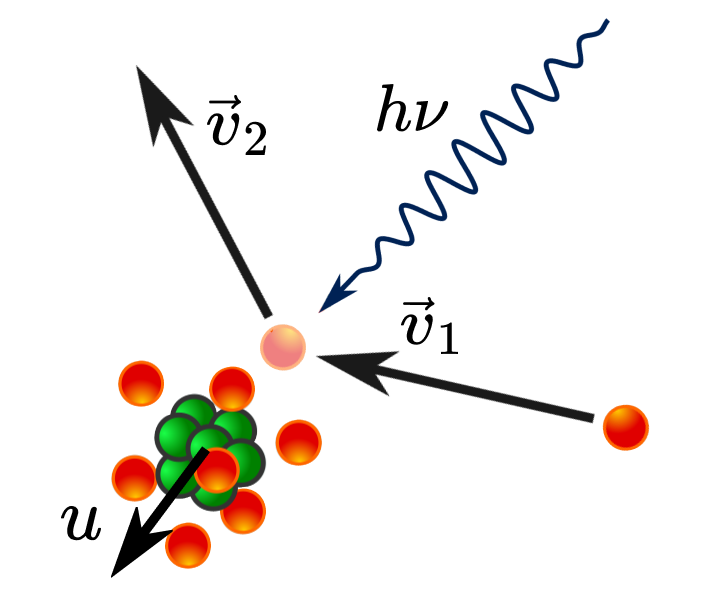
\includegraphics[width=0.8\linewidth]{res/collision_with_recoil.png}
				\caption*{Photon absorption}
			\end{figure}
			
			\column{0.5\linewidth}
			Photon energy is much higher than oscillation energy:
			$$  h\nu = 1.8 \text{ eV} \gg\varepsilon_{\text{osc}} \approx 2.3\cdot 10^{-2} \text{ eV} $$
			\footnotesize
			\emph{(ruby laser, $\omega = 2.7 \cdot 10^{15} \text{ Hz, } E \approx 10^7 \text{ V/cm}$)}
		\end{columns}
		
		Quantum mechanics shows that classic formula conditions can be enhanced:
		\begin{center}
			\boxed{\varepsilon \gg h\nu \gg \varepsilon_{\text{osc}}}
		\end{center}
		
		\footnotesize
		\emph{Electron energy $\varepsilon \approx 10 \text{ eV}$ meet conditions}.
		
		
		
		%		Отметим, что для фотонов не выполняется требование $\varepsilon_{\text{кол}} \approx 2.3\cdot 10^{-2} \text{ эВ} \ll h\nu = 1.8 \text{ эВ}$ (значения для рубинового лазера $\omega = 2.7 \cdot 10^{15} \text{ Гц}, E \approx 10^7 \text{ В/см}$).
		%		t_1^{-1} ln( N_1 / N_0)
		%		Как же быть?
		%		
		%		Столкновения все также остаются важны, так как изолированный электрон не может поглощать фотоны -- это противоречит ЗСИ.
		%		
		%		Поглощение и излучение фотонов электронами при столкновениях -- обратные друг другу процессы с близкими вероятностями, но поглощение происходит немного чаще.
		%		
		%		Более тщательные выкладки с использованием квантовой механики показывают, что классическая формула является применимой в условиях $\varepsilon \gg h\nu$.
		%		Значения $\varepsilon \approx 10 \text{ эВ}$ позволяют применять данную формулу для оценок.
	\end{frame}
	
	\begin{frame}
		\frametitle{Electron energy loss}
		
		There are two types of energy losses: elastic and non-elastic.
		
		\begin{columns}[t]
			\column{0.33\linewidth}
			\begin{figure}
				\centering
				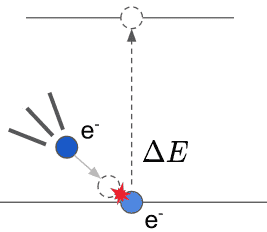
\includegraphics[width=0.8\linewidth]{res/excitation.png}
				\caption*{Excitation by collision}
				
				Non-elastic\\
				$\varepsilon \sim 2/3I \div 3/4I$\\
				(inert gases)
			\end{figure}
			
			\column{0.33\linewidth}
			\vspace{10pt}
			\begin{figure}
				\centering
				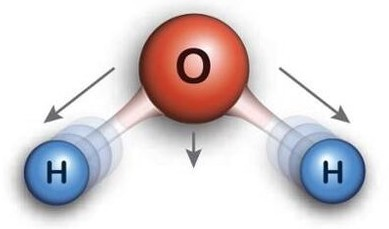
\includegraphics[width=1.0\linewidth]{res/vibrations.jpg}
				\caption*{Molecular vibrations}
				Non-elastic\\
				Whole range of $\varepsilon$\\
				(molecular gases)
			\end{figure}
			
			\column{0.33\linewidth}
			\begin{figure}
				\centering
				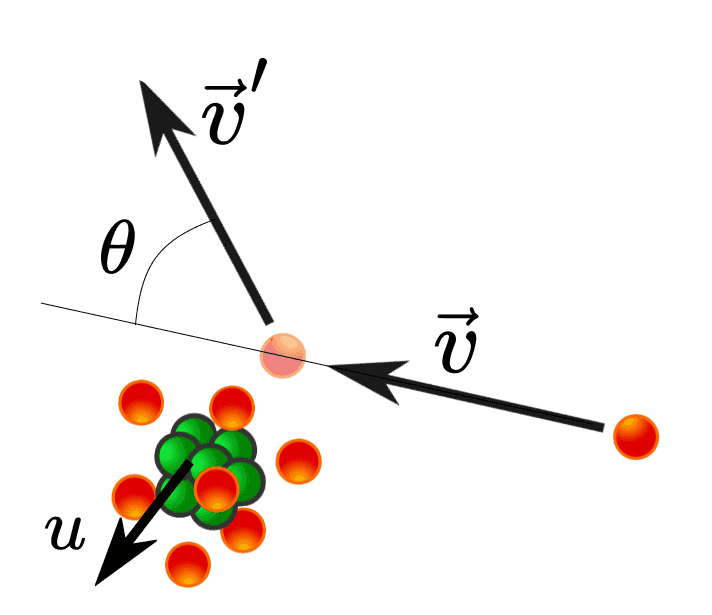
\includegraphics[width=0.8\linewidth]{res/recoil_loss.png}
				\caption*{Collision recoil}
				
				Elastic\\
				All collisions
			\end{figure}
			
		\end{columns}
		
		%		Существует два рода потерь: упругие и неупругие.
		%		
		%		Упругие: отдача части энергии атому при соударении. Роль тем больше, чем легче газ. Работают при всех значениях энергии электрона.
		%		
		%		Неупругие: колебательные состояния молекулярных газов.
		%		Неупругие: Возбуждение атомов. Работают при энергии $2/3I \div 3/4I$ (инертные газы).
		%		
		%		Для лавины (статика, СВЧ) возбуждение атомов губительно, поскольку на зарождении лавины электронов мало и шансов для попадания энергичного (хоть и не достаточно для ионизации невозбужденного) электрона с возбужденным мала.
		%		
		%		Для оптических частот для возбужденных атомов есть повышение вероятности многоквантового фотоэффекта. Но не на всех частотах это действительно улучшает показатели.
		%		
	\end{frame}
	
	\begin{frame}
		\frametitle{Electron losses}
		
		\begin{figure}
			\centering
			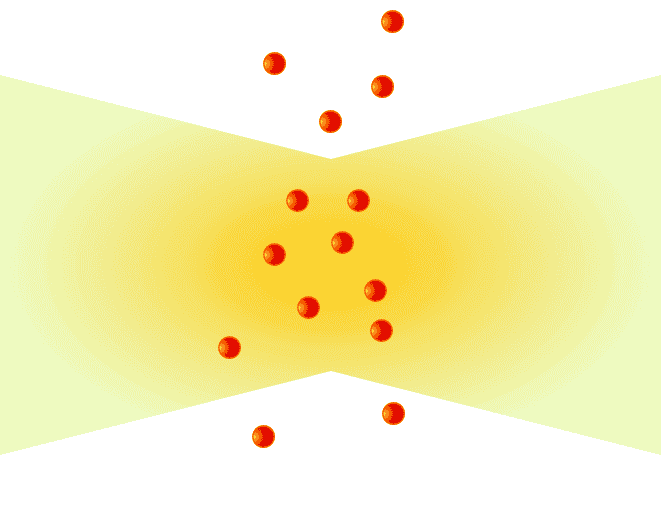
\includegraphics[width=0.5\linewidth]{res/diffusion.png}
			\caption*{Electron diffusion}
		\end{figure}
		
		Main loss mechanism -- diffusion from focus spot.
		
	\end{frame}
	
	\begin{frame}
		\frametitle{Breakdown criterion}
		Electron amount:
		$$ N_e = N_0 e^{\left[(\nu_i - \nu_d) t\right]} = N_0 e^{(t/\theta)},$$
		$\theta = (\nu_i - \nu_d)^{-1}$ -- avalanche time constant,\\
		$\nu_i$ -- electron-atom ionization frequency,\\
		$\nu_d$ -- diffusion loss frequency.
		
		Within impulse time $t_1 \approx 30 \div 50$ ns $N_1 \approx 10^{13}$ electrons should appear:
		
		$$ \theta < \frac{t_1}{\ln( N_1 / N_0)}.$$
		Combining this condition with energy growth $d\varepsilon/dt$:
		\begin{center}
			\boxed{E = \left[\frac{m \omega^2 I}{e^2 \nu_m t_1} \ln \frac{N_1} {N_0}\right]^{1/2}}
		\end{center}
		
		%		Здесь не написано про опускание потерь энергии и потерь электронов: нужно сказать устно.
		%		Также ничего не сказано про N_1 $\approx$ 10^{13}
		
		
		%		Что нам нужно? Нужно, чтобы образовалась лавина.
		%		
		%		Потери энергии и потери электронов определяют пороговое значение поля. При этом потери электронов обрывают цепи электронной лавины, тогда как потери энергии лишь затормаживают развитие лавины.
		%		
		%		$\nu_i$ -- частота ионизации атомов электронами.
		%		$\nu_d$ -- частота диффузионных уходов.
		%		
		%		Частота ионизации без учета потерь энергии
		%		$$ \nu_i = \tau_i^{-1} = \frac{1}{I} \frac{d\varepsilon}{dt}$$.
		%		
		%		$$ \nu_d = \tau_d^{-1} = D / \Lambda^2$$
		%		$\Lambda$ -- диффузионная длина, у нас -- порядка размера пятна (для сферы $r/\pi$)
		%		
		%		Для электронов в зарождении пробоя характерна свободная (самостоятельная) диффузия.
		%		$$ D = l_m v/3 = v^2/3\nu_m$$
		%		$l_m = v / \nu_m$ -- длина пробега электронов.
		%		
		%		Экспоненциальный рост числа электронов:
		%		$$ dN_e/dt = N_e (\nu_i - \nu_d)$$
		%		$$ N_e = N_0 exp\left[(\nu_i - \nu_d) t\right] = N_0 exp(t/\theta)$$
		%		$\theta = (\nu_i - \nu_d)^{-1}$ -- постоянная времени лавины.
		%		
		%		Для статических и СВЧ полей можно принять $\nu_i = \nu_d$ как критерий.
		%		Для оптического диапазона $\theta$ должна быть достаточно малой, чтобы за время импульса $t_1 \approx 3 \cdot 10^{-8}$ с успело образоваться достаточно число электронов.
		%		
		%		Из экспериментов: $\mathfrak{N} \approx 10^{13}$
		%		$k = log_2 10^13 = 43 \Rightarrow \theta = 1 \text{ нс}$, что много меньше времени диффузии.
		%		
		%		В условиях 'нестационарного' пробоя 
		%		$$ \theta^{-1} = t_1^{-1} ln( N_1 / N_0). \text{ ПОЧЕМУ ТУТ ln, а не } log_2?$$
		%		
		%		Рассматривая
		%		1) малые давления (меньше сотен атмосфер, $\omega^2 \gg \nu_m^2$).
		%		2) фокусировка не слишком острая, диффузионные потоки малы.
		%		Совмещая условие пробоя $\theta^{-1} = ...$ и $\frac{d\varepsilon}{dt}$ получаем 
		%		$$ E = \left[\frac{m \omega^2 I_1}{e^2 \nu_m t_1} ln N_1 / N_0\right]^{1/2}$$
		%		
		%		Пороги для молекулярных газов выше, чем атомарных (из-за больших неупругих потерь, 1) на колебательные степени свободы, 2) низкие уровни возбуждения, которые сложно преодолеть).
	\end{frame}
	
	\begin{frame}
		$\nu_m = \nu_c (1 - \overline{\cos{\theta}})$
		$\theta$ -- угол рассеяния.
		
		$(1 - \overline{\cos{\theta}})$ обычно близка к 1 $\Rightarrow$ можно просто брать $\nu_m = \nu_c$?.
		
		$\nu_c = N_a v \sigma_c$, $N_a$ -- число атомов в 1 см$^3$, $v$ -- скорость электрона, $\sigma_c$ -- сечение упругого рассеяния.
		
		Райзер, с53: У гелия частота столкновений почти не зависит от и энергии электронов $v_m \approx 2,4\cdot 10^9 P$ (в торр). Полезно знать, что у водорода зависимость $\nu_m (v)$ также слабая и $\nu_m \approx 5.9 \cdot 10^9 P$ (в торр)
		Аргон: $\nu_m \approx 7 \cdot 10^9 P$ (в торр)
	\end{frame}
	%		TODO: 6 глава, оттуда вытащить более точное значение порога
	%		TODO: Райзер, с53: Рассказывается про асимптотики. Нужно выяснить \nu_m, тогда можно рассказать про асимптотики. Не факт. что очень нужно.
	%		TODO OR NOT TODO: Из кинетического уравнения можно оценить неупругие потери, но оно где-то далеко впереди.
	
	\begin{frame}[plain,c]
		
		\begin{center}
			\huge \usebeamercolor[fg]{frametitle} Измерения и Результаты
		\end{center}
		
	\end{frame}
	
	
	\begin{frame}
		\frametitle{Экспериментальная установка}
		%TODO: обрезать фотку, подписать модули
		\begin{figure}
			\centering
			\includegraphics[width=0.9\linewidth]{res/photodiode_setup.jpg}
			\caption*{Общий вид установки\\ \footnotesize (на переднем фоне система линз для фокусировки вспышки) }
		\end{figure}
	\end{frame}
	
	\begin{frame}
		\frametitle{Экспериментальная установка}
		\begin{figure}
			\centering
			\includegraphics[width=0.9\linewidth]{res/spark_setup.jpg}
			\caption*{Площадка с набором линз для фокусировки пучка}
		\end{figure}
		
	\end{frame}
	
	\begin{frame}
		\frametitle{Спектр воздушного пробоя}
		\begin{figure}
			\centering
			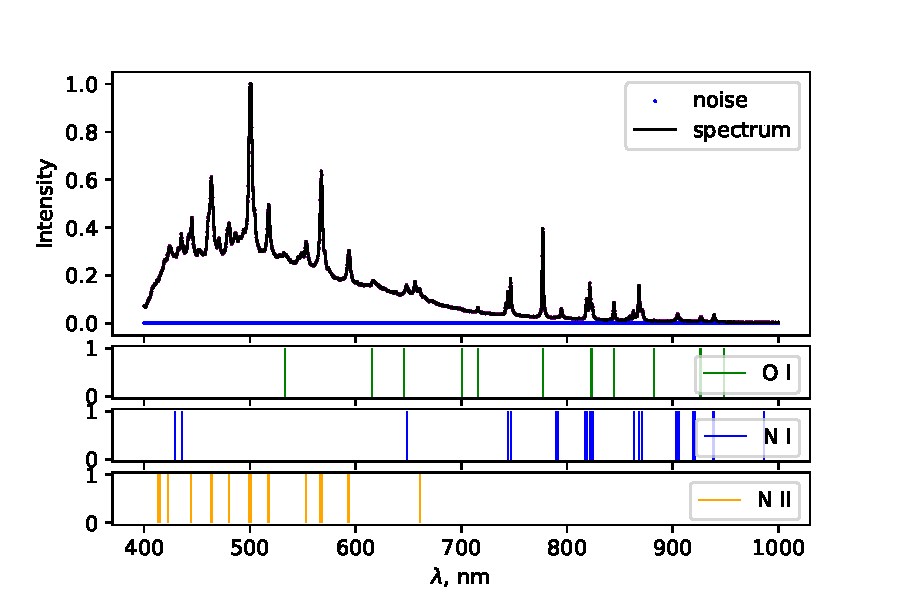
\includegraphics[width=\linewidth]{gen/air_lines.pdf}
			\caption*{Спектр пробоя в воздухе}
		\end{figure}
	\end{frame}
	
	\begin{frame}
		\frametitle{Спектр пробоя ксенона}
		\begin{figure}
			\centering
			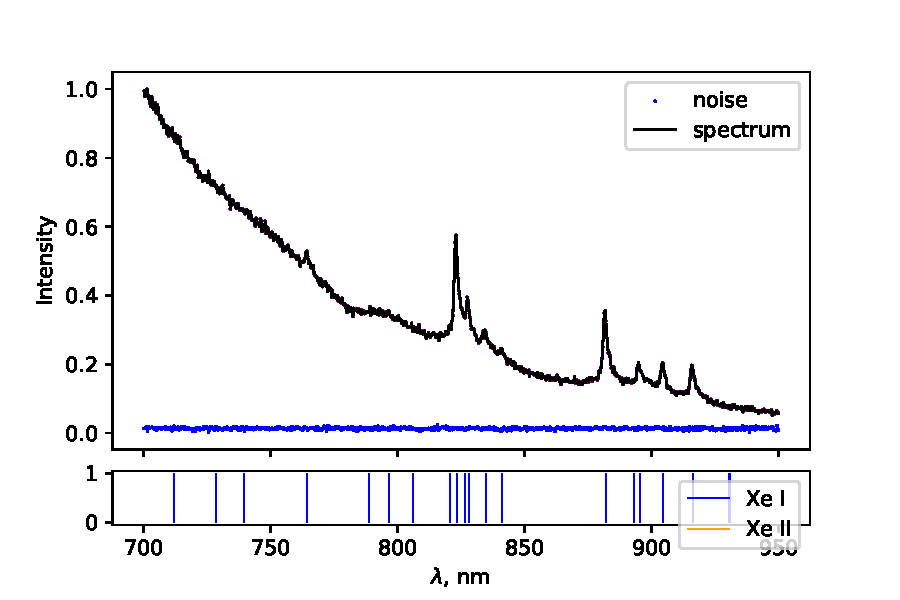
\includegraphics[width=\linewidth]{gen/xe_lines_spherical.pdf}
			\caption*{Спектр пробоя ксенона в шаровой лампе}
		\end{figure}
	\end{frame}
	
	\begin{frame}
		\frametitle{Спектр пробоя ксенона}
		\begin{figure}
			\centering
			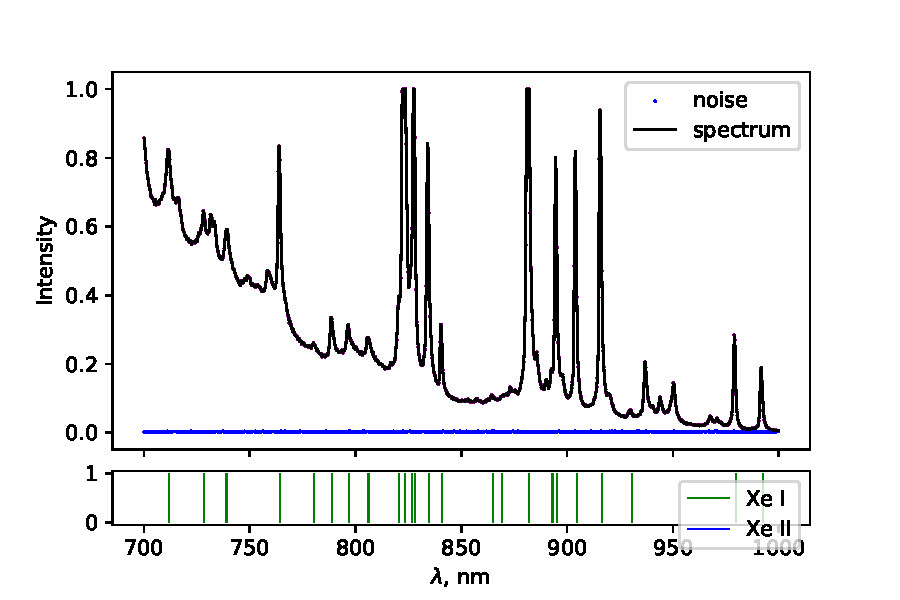
\includegraphics[width=\linewidth]{gen/xe_lines.pdf}
			\caption*{Спектр пробоя ксенона в длинной лампе}
		\end{figure}
	\end{frame}
	
	\begin{frame}
		\frametitle{Спектры}
		
		\begin{center}
			\huge \usebeamercolor[fg]{frametitle} \textit{in progress...}
		\end{center}
		
	\end{frame}
	
	\begin{frame}
		\frametitle{Осциллограммы}
		
		\begin{center}
			\huge \usebeamercolor[fg]{frametitle} \textit{in progress...}
		\end{center}
		
	\end{frame}
	
	\begin{frame}[plain,c]
		
		\begin{center}
			\huge \usebeamercolor[fg]{frametitle} Выводы и Заключение
		\end{center}
		
	\end{frame}
	
	\begin{frame}
		\frametitle{Выводы и Заключение}
		
		\begin{center}
			\huge \usebeamercolor[fg]{frametitle} \textit{in progress...}
		\end{center}
		
	\end{frame}
	
	
	\begin{frame}[plain,c]
		
		\begin{center}
			\huge \usebeamercolor[fg]{frametitle} Спасибо за внимание!
		\end{center}
		
	\end{frame}
	
\end{document}